\subsection{SeafloorAI}
{{\footnotesize
\noindent A first-of-its-kind dataset covering 17,300 sq.km of seafloor with 696K sonar images, 827K segmentation masks, and 696K natural-language descriptions plus \textasciitilde{}7M QA pairs-designed for both vision and language-based ML models in marine science


\begin{description}[labelwidth=4cm, labelsep=1em, leftmargin=4cm, itemsep=0.1em, parsep=0em]
  \item[date:] 2024-12-13
  \item[version:] v1.0
  \item[last\_updated:] 2024-12
  \item[expired:] unknown
  \item[valid:] yes
  \item[valid\_date:] 2024-12-13
  \item[url:] \href{https://neurips.cc/virtual/2024/poster/97432}{https://neurips.cc/virtual/2024/poster/97432}
  \item[doi:] 10.48550/arXiv.2411.00172
  \item[domain:] Marine Science; Vision-Language
  \item[focus:] Large-scale vision-language dataset for seafloor mapping and geological classification
  \item[keywords:]
    - sonar imagery
    - vision-language
    - seafloor mapping
    - segmentation
    - QA
  \item[licensing:] unknown
  \item[task\_types:]
    - Image segmentation
    - Vision-language QA
  \item[ai\_capability\_measured:]
    - Geospatial understanding
    - multimodal reasoning
  \item[metrics:]
    - Segmentation pixel accuracy
    - QA accuracy
  \item[models:]
    - SegFormer
    - ViLT-style multimodal models
  \item[ml\_motif:]
    - Vision-Language
  \item[type:] Dataset
  \item[ml\_task:]
    - Segmentation, QA
  \item[solutions:] Solution details are described in the referenced paper or repository.
  \item[notes:] Data processing code publicly available, covering five geological layers; curated with marine scientists

  \item[contact.name:] Kien X. Nguyen
  \item[contact.email:] unknown
  \item[datasets.links.name:] Sonar imagery + annotations
  \item[datasets.links.url:] \href{unknown}{unknown}
  \item[results.links.name:] ChatGPT LLM
  \item[results.links.url:] \href{unknown}{unknown}
  \item[fair.reproducible:] Yes
  \item[fair.benchmark\_ready:] Yes
  \item[id:] seafloorai
  \item[Citations:] \cite{nguyen2024seafloor}
\end{description}

{\bf Ratings:} ~ \\

\begin{tabular}{p{0.15\textwidth} p{0.07\textwidth} p{0.7\textwidth}}
\hline
Rating & Value & Reason \\
\hline
dataset & 5 & Large-scale, well-annotated sonar imagery dataset with segmentation masks
and natural language descriptions; curated with domain experts.
 \\
documentation & 4 & Dataset description and data processing instructions are provided,
but tutorials and benchmark usage guides are limited.
 \\
metrics & 5 & Standard segmentation pixel accuracy and QA accuracy metrics are clearly specified
and appropriate for the tasks.
 \\
reference\_solution & 4 & Some baseline models (e.g., SegFormer, ViLT-style) are mentioned, but
reproducible code or pretrained weights are not fully available yet.
 \\
software & 3 & Data processing code is publicly available, but no full benchmark framework or
runnable model implementations are provided yet.
 \\
specification & 5 & Tasks (image segmentation and vision-language QA) are clearly defined with
geospatial and multimodal objectives well specified.
 \\
\hline
\end{tabular}

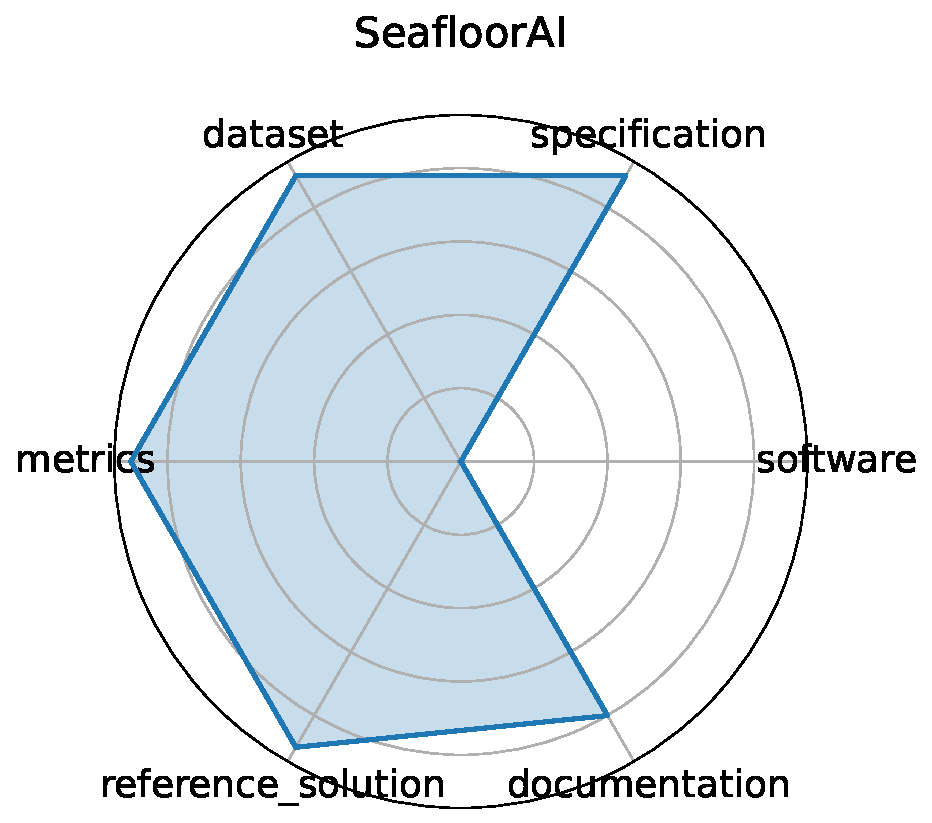
\includegraphics[width=0.2\textwidth]{seafloorai_radar.pdf}
}}
\clearpage